% Options for packages loaded elsewhere
\PassOptionsToPackage{unicode}{hyperref}
\PassOptionsToPackage{hyphens}{url}
\PassOptionsToPackage{dvipsnames,svgnames,x11names}{xcolor}
%
\documentclass[
  letterpaper,
  DIV=11,
  numbers=noendperiod]{scrartcl}

\usepackage{amsmath,amssymb}
\usepackage{lmodern}
\usepackage{iftex}
\ifPDFTeX
  \usepackage[T1]{fontenc}
  \usepackage[utf8]{inputenc}
  \usepackage{textcomp} % provide euro and other symbols
\else % if luatex or xetex
  \usepackage{unicode-math}
  \defaultfontfeatures{Scale=MatchLowercase}
  \defaultfontfeatures[\rmfamily]{Ligatures=TeX,Scale=1}
\fi
% Use upquote if available, for straight quotes in verbatim environments
\IfFileExists{upquote.sty}{\usepackage{upquote}}{}
\IfFileExists{microtype.sty}{% use microtype if available
  \usepackage[]{microtype}
  \UseMicrotypeSet[protrusion]{basicmath} % disable protrusion for tt fonts
}{}
\makeatletter
\@ifundefined{KOMAClassName}{% if non-KOMA class
  \IfFileExists{parskip.sty}{%
    \usepackage{parskip}
  }{% else
    \setlength{\parindent}{0pt}
    \setlength{\parskip}{6pt plus 2pt minus 1pt}}
}{% if KOMA class
  \KOMAoptions{parskip=half}}
\makeatother
\usepackage{xcolor}
\usepackage[top=30mm,left=30mm]{geometry}
\setlength{\emergencystretch}{3em} % prevent overfull lines
\setcounter{secnumdepth}{-\maxdimen} % remove section numbering
% Make \paragraph and \subparagraph free-standing
\ifx\paragraph\undefined\else
  \let\oldparagraph\paragraph
  \renewcommand{\paragraph}[1]{\oldparagraph{#1}\mbox{}}
\fi
\ifx\subparagraph\undefined\else
  \let\oldsubparagraph\subparagraph
  \renewcommand{\subparagraph}[1]{\oldsubparagraph{#1}\mbox{}}
\fi

\usepackage{color}
\usepackage{fancyvrb}
\newcommand{\VerbBar}{|}
\newcommand{\VERB}{\Verb[commandchars=\\\{\}]}
\DefineVerbatimEnvironment{Highlighting}{Verbatim}{commandchars=\\\{\}}
% Add ',fontsize=\small' for more characters per line
\usepackage{framed}
\definecolor{shadecolor}{RGB}{241,243,245}
\newenvironment{Shaded}{\begin{snugshade}}{\end{snugshade}}
\newcommand{\AlertTok}[1]{\textcolor[rgb]{0.68,0.00,0.00}{#1}}
\newcommand{\AnnotationTok}[1]{\textcolor[rgb]{0.37,0.37,0.37}{#1}}
\newcommand{\AttributeTok}[1]{\textcolor[rgb]{0.40,0.45,0.13}{#1}}
\newcommand{\BaseNTok}[1]{\textcolor[rgb]{0.68,0.00,0.00}{#1}}
\newcommand{\BuiltInTok}[1]{\textcolor[rgb]{0.00,0.23,0.31}{#1}}
\newcommand{\CharTok}[1]{\textcolor[rgb]{0.13,0.47,0.30}{#1}}
\newcommand{\CommentTok}[1]{\textcolor[rgb]{0.37,0.37,0.37}{#1}}
\newcommand{\CommentVarTok}[1]{\textcolor[rgb]{0.37,0.37,0.37}{\textit{#1}}}
\newcommand{\ConstantTok}[1]{\textcolor[rgb]{0.56,0.35,0.01}{#1}}
\newcommand{\ControlFlowTok}[1]{\textcolor[rgb]{0.00,0.23,0.31}{#1}}
\newcommand{\DataTypeTok}[1]{\textcolor[rgb]{0.68,0.00,0.00}{#1}}
\newcommand{\DecValTok}[1]{\textcolor[rgb]{0.68,0.00,0.00}{#1}}
\newcommand{\DocumentationTok}[1]{\textcolor[rgb]{0.37,0.37,0.37}{\textit{#1}}}
\newcommand{\ErrorTok}[1]{\textcolor[rgb]{0.68,0.00,0.00}{#1}}
\newcommand{\ExtensionTok}[1]{\textcolor[rgb]{0.00,0.23,0.31}{#1}}
\newcommand{\FloatTok}[1]{\textcolor[rgb]{0.68,0.00,0.00}{#1}}
\newcommand{\FunctionTok}[1]{\textcolor[rgb]{0.28,0.35,0.67}{#1}}
\newcommand{\ImportTok}[1]{\textcolor[rgb]{0.00,0.46,0.62}{#1}}
\newcommand{\InformationTok}[1]{\textcolor[rgb]{0.37,0.37,0.37}{#1}}
\newcommand{\KeywordTok}[1]{\textcolor[rgb]{0.00,0.23,0.31}{#1}}
\newcommand{\NormalTok}[1]{\textcolor[rgb]{0.00,0.23,0.31}{#1}}
\newcommand{\OperatorTok}[1]{\textcolor[rgb]{0.37,0.37,0.37}{#1}}
\newcommand{\OtherTok}[1]{\textcolor[rgb]{0.00,0.23,0.31}{#1}}
\newcommand{\PreprocessorTok}[1]{\textcolor[rgb]{0.68,0.00,0.00}{#1}}
\newcommand{\RegionMarkerTok}[1]{\textcolor[rgb]{0.00,0.23,0.31}{#1}}
\newcommand{\SpecialCharTok}[1]{\textcolor[rgb]{0.37,0.37,0.37}{#1}}
\newcommand{\SpecialStringTok}[1]{\textcolor[rgb]{0.13,0.47,0.30}{#1}}
\newcommand{\StringTok}[1]{\textcolor[rgb]{0.13,0.47,0.30}{#1}}
\newcommand{\VariableTok}[1]{\textcolor[rgb]{0.07,0.07,0.07}{#1}}
\newcommand{\VerbatimStringTok}[1]{\textcolor[rgb]{0.13,0.47,0.30}{#1}}
\newcommand{\WarningTok}[1]{\textcolor[rgb]{0.37,0.37,0.37}{\textit{#1}}}

\providecommand{\tightlist}{%
  \setlength{\itemsep}{0pt}\setlength{\parskip}{0pt}}\usepackage{longtable,booktabs,array}
\usepackage{calc} % for calculating minipage widths
% Correct order of tables after \paragraph or \subparagraph
\usepackage{etoolbox}
\makeatletter
\patchcmd\longtable{\par}{\if@noskipsec\mbox{}\fi\par}{}{}
\makeatother
% Allow footnotes in longtable head/foot
\IfFileExists{footnotehyper.sty}{\usepackage{footnotehyper}}{\usepackage{footnote}}
\makesavenoteenv{longtable}
\usepackage{graphicx}
\makeatletter
\def\maxwidth{\ifdim\Gin@nat@width>\linewidth\linewidth\else\Gin@nat@width\fi}
\def\maxheight{\ifdim\Gin@nat@height>\textheight\textheight\else\Gin@nat@height\fi}
\makeatother
% Scale images if necessary, so that they will not overflow the page
% margins by default, and it is still possible to overwrite the defaults
% using explicit options in \includegraphics[width, height, ...]{}
\setkeys{Gin}{width=\maxwidth,height=\maxheight,keepaspectratio}
% Set default figure placement to htbp
\makeatletter
\def\fps@figure{htbp}
\makeatother

\KOMAoption{captions}{tableheading}
\makeatletter
\makeatother
\makeatletter
\makeatother
\makeatletter
\@ifpackageloaded{caption}{}{\usepackage{caption}}
\AtBeginDocument{%
\ifdefined\contentsname
  \renewcommand*\contentsname{Table of contents}
\else
  \newcommand\contentsname{Table of contents}
\fi
\ifdefined\listfigurename
  \renewcommand*\listfigurename{List of Figures}
\else
  \newcommand\listfigurename{List of Figures}
\fi
\ifdefined\listtablename
  \renewcommand*\listtablename{List of Tables}
\else
  \newcommand\listtablename{List of Tables}
\fi
\ifdefined\figurename
  \renewcommand*\figurename{Figure}
\else
  \newcommand\figurename{Figure}
\fi
\ifdefined\tablename
  \renewcommand*\tablename{Table}
\else
  \newcommand\tablename{Table}
\fi
}
\@ifpackageloaded{float}{}{\usepackage{float}}
\floatstyle{ruled}
\@ifundefined{c@chapter}{\newfloat{codelisting}{h}{lop}}{\newfloat{codelisting}{h}{lop}[chapter]}
\floatname{codelisting}{Listing}
\newcommand*\listoflistings{\listof{codelisting}{List of Listings}}
\makeatother
\makeatletter
\@ifpackageloaded{caption}{}{\usepackage{caption}}
\@ifpackageloaded{subcaption}{}{\usepackage{subcaption}}
\makeatother
\makeatletter
\@ifpackageloaded{tcolorbox}{}{\usepackage[many]{tcolorbox}}
\makeatother
\makeatletter
\@ifundefined{shadecolor}{\definecolor{shadecolor}{rgb}{.97, .97, .97}}
\makeatother
\makeatletter
\makeatother
\ifLuaTeX
  \usepackage{selnolig}  % disable illegal ligatures
\fi
\IfFileExists{bookmark.sty}{\usepackage{bookmark}}{\usepackage{hyperref}}
\IfFileExists{xurl.sty}{\usepackage{xurl}}{} % add URL line breaks if available
\urlstyle{same} % disable monospaced font for URLs
\hypersetup{
  pdftitle={Neural Network Maths},
  pdfauthor={Thomas Simm},
  colorlinks=true,
  linkcolor={blue},
  filecolor={Maroon},
  citecolor={Blue},
  urlcolor={Blue},
  pdfcreator={LaTeX via pandoc}}

\title{Neural Network Maths}
\author{Thomas Simm}
\date{}

\begin{document}
\maketitle
\ifdefined\Shaded\renewenvironment{Shaded}{\begin{tcolorbox}[boxrule=0pt, borderline west={3pt}{0pt}{shadecolor}, enhanced, breakable, interior hidden, frame hidden, sharp corners]}{\end{tcolorbox}}\fi

\renewcommand*\contentsname{Table of contents}
{
\hypersetup{linkcolor=}
\setcounter{tocdepth}{3}
\tableofcontents
}
\begin{Shaded}
\begin{Highlighting}[]
\CommentTok{\#hide}
\ImportTok{import}\NormalTok{ tensorflow }\ImportTok{as}\NormalTok{ tf}
\ImportTok{import}\NormalTok{ numpy }\ImportTok{as}\NormalTok{ np}
\ImportTok{import}\NormalTok{ matplotlib.pyplot }\ImportTok{as}\NormalTok{ plt}
\end{Highlighting}
\end{Shaded}

\hypertarget{gradient-descent}{%
\subsection{Gradient Descent}\label{gradient-descent}}

Gradient descent is an algroithm used to determine the value of
parameters that are used to map input variables to target variables. The
steps are: - Determine a loss function that relates predictions and
actual values, i.e.~a function that determines how good the predictions
are - N.B. the function needs to be of a form to encourage gradient
descent - Find the gradient of the loss function with respect to the
parameters - Update the weights based on this gradient

For example, in the figure below - if the weight W=0 then the Loss is 1
and the gradient is -1.0. In this case we'd want to increase the value
of the weight W towards it's minimum 0.5 - if the weight W=1 then the
Loss is also 1 but the gradient is +1.0. In this case we'd want to
reduce the value of the weight W towards it's minimum 0.5 - if the
weight W=0.5 then the loss is close 0 and so is the garient, in this
case we wouldn't want to change the weights by much

i.e.~the weights can be updated by a formula of the form below to get
the best fit:

\[W_{i+1} = W_i - const . \frac{dJ}{dW}\]

\begin{quote}
Gradient descent is not the only optimisation method to determine
parameters but is an easy one to understand.
\end{quote}

\begin{Shaded}
\begin{Highlighting}[]
\CommentTok{\#hide{-}input}
\NormalTok{xx}\OperatorTok{=}\NormalTok{np.arange(}\DecValTok{0}\NormalTok{,np.pi,}\FloatTok{.1}\NormalTok{)}
\NormalTok{plt.plot(xx}\OperatorTok{/}\NormalTok{np.pi,}\DecValTok{1}\OperatorTok{+}\NormalTok{np.sin(}\OperatorTok{{-}}\NormalTok{xx),}\StringTok{\textquotesingle{}{-}k\textquotesingle{}}\NormalTok{,linewidth}\OperatorTok{=}\DecValTok{4}\NormalTok{)}
\NormalTok{plt.plot(xx}\OperatorTok{/}\NormalTok{np.pi,}\OperatorTok{{-}}\NormalTok{np.cos(}\OperatorTok{{-}}\NormalTok{xx),}\StringTok{\textquotesingle{}k{-}{-}\textquotesingle{}}\NormalTok{,linewidth}\OperatorTok{=}\DecValTok{4}\NormalTok{)}
\NormalTok{plt.legend([}\StringTok{\textquotesingle{}Loss Function J\textquotesingle{}}\NormalTok{,}\StringTok{\textquotesingle{}Gradient dJ/dW\textquotesingle{}}\NormalTok{])}
\NormalTok{plt.xlabel(}\StringTok{\textquotesingle{}W\textquotesingle{}}\NormalTok{)}
\NormalTok{plt.ylabel(}\StringTok{\textquotesingle{}J\textquotesingle{}}\NormalTok{)}
\NormalTok{plt.grid(}\VariableTok{True}\NormalTok{)}
\end{Highlighting}
\end{Shaded}

\begin{figure}[H]

{\centering 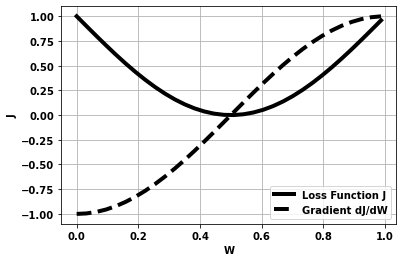
\includegraphics{2022-10-10-NeuralNetworksMaths_files/figure-pdf/cell-3-output-1.png}

}

\end{figure}

Some definitions.

\begin{itemize}
\tightlist
\item
  \texttt{X} are the input variables
\item
  \texttt{Y} the target variables
\item
  \(\hat{y}\) is the prediction
\item
  The loss function \texttt{J} is what we are trying to minimise and is
  the sum of \({Y-\hat{y}^2}\). For simplicity we'll remove the
  summation below.
\item
  \texttt{m} and \texttt{b} are the parameters we are looking to obtain
\end{itemize}

\(\hat{Y}= mX +b\)

\(Error = \hat{Y} - Y\)

\(J(m,b) = Error^2\)

\(Error = mX + b - Y\)

What we want to do is update \texttt{m} and \texttt{b} so that
\texttt{J} is reduced and the predictions is better. That is for
\texttt{m} we obtain a new value (1) from the previous one (0) as
follows:

\(m_1 = m_0 - \frac{dJ}{dm} . \alpha\)

Where we have also included a learning rate (\(\alpha\)\textless1) to
make the changes smoother.

So to improve the predictions of the model we need to find \frac{dJ}{dm}
and \frac{dJ}{db}. Which involves a bit of differentiation and
rearanging as follows.

Chain rule for differentiation to find \texttt{db} and \texttt{dm}

\(\frac{dJ}{dm}\ = \frac{dJ}{dError}\ \frac{dError}{dm}\)

\(\frac{dJ}{db}\ = \frac{dJ}{dError}\ \frac{dError}{db}\)

from definition of J

\(\frac{dJ}{dError}\ = 2 . Error\)

from definition of Error

\(\frac{dError}{dm} = X\)

\(\frac{dError}{db} = 1\)

So

\(\frac{dJ}{dm} = 2 . Error . X\)

\(\frac{dJ}{db} = 2 . Error . 1\)

And to account for the summation we divide by the length of the array.

To allow for matrix multiplication we create \texttt{X} as a matrix of
two vectors one with just ones and the 2nd part the original X. This
then allows us to have one variable for the weights \texttt{m} and
\texttt{b} that we are fitting to.

So for each iteration (\texttt{K}) the weights \texttt{W} (\texttt{j}
are the different parts to the weights e.g.~\texttt{b} and \texttt{m})
are updated. Noting that there are \texttt{N} observations (length of y
is N) we get:

\(W_j^{K+1} = W_j^{K} - [\alpha . \frac{1}{N}\sum(\hat{Y}-Y).X_j]\)

\begin{Shaded}
\begin{Highlighting}[]
\KeywordTok{def}\NormalTok{ computeCost(X,y, theta):}
\NormalTok{    Ypred }\OperatorTok{=}\NormalTok{ np.matmul(X,theta)}
\NormalTok{    J }\OperatorTok{=}\NormalTok{np.}\BuiltInTok{sum}\NormalTok{( (}\DecValTok{1}\OperatorTok{/}\NormalTok{(}\DecValTok{2}\OperatorTok{*}\BuiltInTok{len}\NormalTok{(y)))}\OperatorTok{*}\NormalTok{ (Ypred }\OperatorTok{{-}}\NormalTok{ y)}\OperatorTok{**}\DecValTok{2}\NormalTok{ )}
    \ControlFlowTok{return}\NormalTok{ J,Ypred}
\KeywordTok{def}\NormalTok{ computeGrad(X, y, theta,learningRate):}
\NormalTok{    J,Ypred }\OperatorTok{=}\NormalTok{ computeCost(X,y, theta)}
\NormalTok{    error }\OperatorTok{=}\NormalTok{ (Ypred }\OperatorTok{{-}}\NormalTok{ y)}\OperatorTok{*}\NormalTok{learningRate}\OperatorTok{/}\BuiltInTok{len}\NormalTok{(y)}
    \ControlFlowTok{return}\NormalTok{ [np.}\BuiltInTok{sum}\NormalTok{(error),np.}\BuiltInTok{sum}\NormalTok{(X[:,}\DecValTok{1}\NormalTok{]}\OperatorTok{*}\NormalTok{error)], J}
    
\end{Highlighting}
\end{Shaded}

Create the variables to fit to

\begin{Shaded}
\begin{Highlighting}[]
\NormalTok{X }\OperatorTok{=}\NormalTok{ np.ones((}\DecValTok{50}\NormalTok{,}\DecValTok{2}\NormalTok{))}
\NormalTok{X[:,}\DecValTok{1}\NormalTok{]}\OperatorTok{=}\NormalTok{np.arange(}\DecValTok{0}\NormalTok{,}\DecValTok{1}\NormalTok{,}\FloatTok{.02}\NormalTok{)}
\NormalTok{theta\_act }\OperatorTok{=}\NormalTok{ [}\FloatTok{.5}\NormalTok{,}\DecValTok{3}\NormalTok{]}
\NormalTok{y }\OperatorTok{=}\NormalTok{ np.matmul(X,theta\_act)}
\NormalTok{plt.plot(X[:,}\DecValTok{0}\NormalTok{],y,}\StringTok{\textquotesingle{}.r\textquotesingle{}}\NormalTok{)}
\NormalTok{plt.plot(X[:,}\DecValTok{1}\NormalTok{],y,}\StringTok{\textquotesingle{}.k\textquotesingle{}}\NormalTok{)}
\NormalTok{plt.grid(}\VariableTok{True}\NormalTok{)}
\NormalTok{plt.title(}\StringTok{\textquotesingle{}Data\textquotesingle{}}\NormalTok{)}
\NormalTok{plt.legend([}\StringTok{\textquotesingle{}bias b\textquotesingle{}}\NormalTok{,}\StringTok{\textquotesingle{}m gradient\textquotesingle{}}\NormalTok{])}\OperatorTok{;}
\NormalTok{plt.xlabel(}\StringTok{\textquotesingle{}X\textquotesingle{}}\NormalTok{)}
\NormalTok{plt.ylabel(}\StringTok{\textquotesingle{}y\textquotesingle{}}\NormalTok{)}\OperatorTok{;}
\end{Highlighting}
\end{Shaded}

\begin{figure}[H]

{\centering 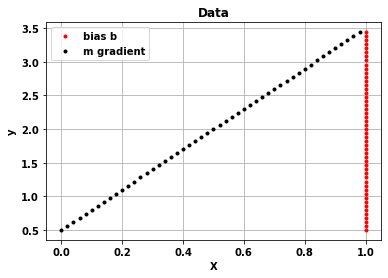
\includegraphics{2022-10-10-NeuralNetworksMaths_files/figure-pdf/cell-5-output-1.png}

}

\end{figure}

Use the gradient descent iteration

\begin{Shaded}
\begin{Highlighting}[]
\NormalTok{theta\_}\OperatorTok{=}\NormalTok{np.array([}\OperatorTok{{-}}\DecValTok{1}\NormalTok{, }\OperatorTok{{-}}\DecValTok{10}\NormalTok{])}
\NormalTok{thetaALL}\OperatorTok{=}\NormalTok{[]}\OperatorTok{;}\NormalTok{ jALL}\OperatorTok{=}\NormalTok{[]}
\NormalTok{iterTot}\OperatorTok{=}\DecValTok{100}
\ControlFlowTok{for}\NormalTok{ \_ }\KeywordTok{in} \BuiltInTok{range}\NormalTok{(iterTot):}
\NormalTok{    thetaALL.append( theta\_ )}
\NormalTok{    (deltaTheta, J) }\OperatorTok{=}\NormalTok{computeGrad(X, y, theta\_,learningRate}\OperatorTok{=}\FloatTok{.5}\NormalTok{)}
\NormalTok{    theta\_ }\OperatorTok{=}\NormalTok{ theta\_ }\OperatorTok{{-}}\NormalTok{ deltaTheta}
    
\NormalTok{    jALL.append(J)}

\NormalTok{plt.plot(}\BuiltInTok{range}\NormalTok{(iterTot),thetaALL,}\StringTok{\textquotesingle{}.{-}\textquotesingle{}}\NormalTok{)}
\NormalTok{plt.plot(}\BuiltInTok{range}\NormalTok{(iterTot),np.ones((iterTot,}\DecValTok{2}\NormalTok{))}\OperatorTok{*}\NormalTok{theta\_act,}\StringTok{\textquotesingle{}{-}{-}\textquotesingle{}}\NormalTok{,linewidth}\OperatorTok{=}\DecValTok{4}\NormalTok{)}
\CommentTok{\# plt.plot(range(iterTot),jALL,\textquotesingle{}:\textquotesingle{},linewidth=4)}
\NormalTok{plt.grid(}\VariableTok{True}\NormalTok{)}
\NormalTok{plt.legend([}\StringTok{\textquotesingle{}b\textquotesingle{}}\NormalTok{,}\StringTok{\textquotesingle{}m\textquotesingle{}}\NormalTok{,}\StringTok{\textquotesingle{}actual values b\textquotesingle{}}\NormalTok{,}\StringTok{\textquotesingle{}actual values m\textquotesingle{}}\NormalTok{,}\StringTok{\textquotesingle{}Loss\textquotesingle{}}\NormalTok{])}
\NormalTok{plt.xlabel(}\StringTok{\textquotesingle{}Iteration\textquotesingle{}}\NormalTok{)}
\NormalTok{plt.ylabel(}\StringTok{\textquotesingle{}Values\textquotesingle{}}\NormalTok{)}\OperatorTok{;}

\end{Highlighting}
\end{Shaded}

\begin{figure}[H]

{\centering 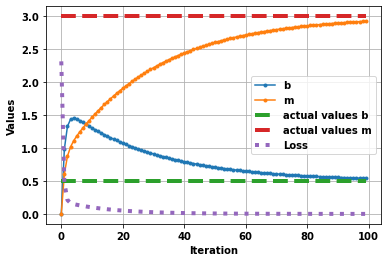
\includegraphics{2022-10-10-NeuralNetworksMaths_files/figure-pdf/cell-6-output-1.png}

}

\end{figure}



\end{document}
